\documentclass[11pt,titlepage,openright]{book}
\usepackage[utf8]{inputenc}
\usepackage[T1]{fontenc}
\usepackage[british]{babel}
\usepackage{graphicx}
\usepackage[dvipsnames]{xcolor}
\usepackage{libertine}
\renewcommand*\ttdefault{cmtt}

\usepackage[sf]{titlesec}
\usepackage[square]{natbib}
\setcitestyle{numbers} 
%\usepackage[export]{adjustbox}

\usepackage{
  paralist,   % Improved lists 
  marginnote, % Improved margin notes
  environ,
  ragged2e,   % Justified text in the margin notes
  url,        % For typesetting URLs
  listings,   % Code formatting
  hyperref,   % Links in PDF from TOC, refs, etc.
  lipsum
}
\usepackage{changepage}
\usepackage{float}

\usepackage[twoside,labelfont=sf]{caption}

\graphicspath{{images/}}

\captionsetup{justification=raggedright,singlelinecheck=false}

\newcommand\myhrulefill[1]{\leavevmode\leaders\hrule height#1\hfill\kern0pt}
\DeclareCaptionFormat{FigFormat}{{\color{black}\myhrulefill{0.5pt}}\\#1#2#3}
%\captionsetup[figure]{format=FigFormat}
%\captionsetup[table]{format=FigFormat}

\DeclareCaptionFormat{LstFormat}{\textsf{Listing}~\arabic{chapter}.\arabic{listing}:#2#3}
\floatstyle{ruled}
\newfloat{listing}{thp}{lol}
\floatname{listing}{Listing}
%\captionsetup[listing]{format=LstFormat}


\NewEnviron{MarginNote}[1][0mm]{\marginnote{\footnotesize\justifying\BODY}[#1]}
\newcommand{\Footnote}[2][0mm]{\footnotemark\marginnote{\footnotesize$^{\arabic{footnote})}$~#2}[#1]}

\renewenvironment{figure*}[1][]{%
  \begin{figure}[#1]%
    \checkoddpage%
    \ifoddpage%
      \begin{adjustwidth}{0cm}{-45mm}%%
    \else%
      \begin{adjustwidth}{-45mm}{0cm}%%
    \fi%
    }{%
    \end{adjustwidth}%
  \end{figure}}

\renewenvironment{table*}[1][]{%
  \begin{table}[#1]%
    \checkoddpage%
    \ifoddpage%
      \begin{adjustwidth}{0cm}{-45mm}%%
    \else%
      \begin{adjustwidth}{-45mm}{0cm}%%
    \fi%
    }{%
    \end{adjustwidth}%
  \end{table}}

\renewenvironment{listing*}[1][]{%
  \begin{listing}[#1]%
    \checkoddpage%
    \ifoddpage%
      \begin{adjustwidth}{0cm}{-45mm}%%
    \else%
      \begin{adjustwidth}{-45mm}{0cm}%%
    \fi%
    }{%
    \end{adjustwidth}%
  \end{listing}}

%% == Code =======================================================
\lstnewenvironment{Code}[1][style=std]{\lstset{#1}}{}
\lstnewenvironment{Code_Numbered}[1][style=std,numbers=left]{\lstset{#1}}{}

\renewcommand{\c}[1]{\lstinline[style=std]@#1@}

\lstdefinestyle{std}{
  language=java,
  basicstyle=\small\sf\color{black},
  keywordstyle=\small\sf\bfseries,
  numberstyle=\footnotesize\sf\color{black},
  commentstyle=\small\color{black}\it,
  aboveskip=1ex,
  belowskip=1ex,
  tabsize=2,
  columns=fullflexible,
  xleftmargin=1ex,
  resetmargins=true,
  showstringspaces=false,
  morecomment=[l]{//},
  morecomment=[l]{--},
  morecomment=[s]{/*}{*/},
  escapeinside=@@,
  morekeywords={Frobies},
  moredelim=[is][\textit]{___}{___},
  moredelim=[is][\textbf]{__*}{*__}
}

\usepackage[activate={true,nocompatibility},final,tracking=true,kerning=true,spacing=false,factor=1100,stretch=10,shrink=10]{microtype}
\usepackage[paper=a4paper,text={13cm,24cm},marginparsep=5mm,marginparwidth=45mm,inner=20mm,twoside]{geometry}

\newcommand{\RED}[1]{\textcolor{red}{#1}}
\newcommand{\ie}{\emph{i.e.,}}
\newcommand{\eg}{\emph{e.g.,}}
\newcommand{\etal}{\emph{et~al.}}

\renewcommand{\bfdefault}{b}
\clearpage{\pagestyle{empty}\cleardoublepage}

\synctex=1
\pagestyle{plain}

\begin{document}
\frontmatter
\title{Implementing NB-IoT: Communication with a Loading Cell}
\author{Johannes Almroth}
\date{\today}

\maketitle

\vspace*{3cm}
\section*{Abstract}
The purpose of this project is to establish a line of communication between a loading cell and the internet. This will be done through the NB-IoT technology, and the data being sent is the one being produced by the loading cell. Using a development board from PyCom and a SIM-card from Telia as the network service provider, [...]


\tableofcontents
%\listoffigures
%\listoftables

\mainmatter

\chapter{Introduction}
% Should be 25% of the total paper

Vetek is a Swedish scale supplier located in Väddö, situated approx. 100 kilometers north of Stockholm. Vetek constructs their own scales and weighing systems, as well as reselling products from other manufacturers.\cite{vetek} 

Vetek aims to improve their services, and as such are interested in the possible use cases of IoT (Internet of Things) technology, and ultimately see how that can be applied to their own products. In this paper,the term IoT will simply mean ``(a) device(s) connected to the internet''\cite{what_is_iot}. In a pilot project, Vetek wants to see how this connectivity can be implemented in a energy-efficient and effective manner. This would entail investigating factors such as power consumption, range and data rate. NB-IoT (Narrowband-IoT), a new and emerging radio technology, encapsulates some principles suitable for this type of endeavor, such as wide coverage, low power consumption and low complexity.\cite{NB-overview} Using some form of NB-IoT compatible microcontroller and hooking it up to a basic load cell should provide sufficient testing grounds to see how this new functionality could improve existing products.


\section{Purpose and Goals}
\iffalse
\begin{itemize}
	\item Write about the grand scheme of things
	\item Set the correct expectations
	\item What can I expect to learn if I keep on reading?
	\item What are the success criteria for this work?
	\item How will the work be evaluated?
\end{itemize}
\fi

NB-IoT is a relatively new technology, and as such, implementations and documentations remain sparse. With this in mind, even a small project such as this will serve as a guiding post for future work. The goal of this project is to establish a working internet connection with a load cell through the NB-IoT technology. The data sent from the load cell should be functionally identical to the data produced if the load cell was offline. Disregarding problems due to a internet service provider, data speeds and losses should not be abnormal. Using the same components, replication of the project should be feasible with the documentation provided in this thesis, assuming software and service providers remain.

The end-goal can be divided into two sub-goals. 
\begin{itemize}
	\item Enable internet communication from the microcontroller.
	\item Enable data transfer from the load cell to the microcontroller.
\end{itemize}


\section{Delimitations}
\iffalse
\begin{itemize}
	\item Scale down expectations and clarify
\end{itemize}
\fi
The final implementation will not be a functional product ready to be used. Any extra improvements upon a internet-enabled load cell will only be done if time remains after the implementation and the completion of the thesis.

\chapter{Background}
% Should be ~2 pages 

% **Problems**

% - Too much mixed information
% - The expensive stuff is not expensive
% - Requirements should be its own chapter

% **Needs to contain**

% - More subheadings

% **Structure**

% - General Background
% - LTE-M vs NB-IoT
% - Market in Sweden

\section{General Background}
IoT has been lauded as a world-changing technology that will significantly affect our economy as well as our way of living. In a report by the GSMA, the total number of IoT devices is estimated to triple by 2025, bringing it to \$25.2 \textit{billion}.\cite{gsma-report} Meanwhile, the global IoT revenue will fourfold from 2018, increasing it to \$4.4 \textit{billion}.\cite{gsma-report} While there undeniably is a lot of excitement and potential economic impact associated with IoT, currently, many consumers just associate the term with connecting a common toaster or coffee machine to a Wi-Fi network. While this technically fits the definition for an IoT device,\cite{what_is_iot} the significant use cases will probably be implemented with different sensors, such as scales, thermometers, etc. that will further improve automatization and optimization processes. As an example, the key categories within the predicted growth are smart homes (\eg~ security devices) and smart buildings (\eg~ energy consumption sensors).\cite{gsma-report} For the predicted growth to happen, businesses need to take a chance and work on projects that implement different IoT technologies, and to enable this, the 3GPP has developed some Low-Power Wide-Area Network (LPWAN) protocols that focus on different key aspects that make IoT possible. Some of these aspect include long battery life, high connection density, indoor coverage and geo-tracking capabilities. Aside from security, one of the biggest challenges regarding IoT devices relate to limitations arising from energy infrastructure. As mentioned earlier, one of the core issues NB-IoT aims to achieve is to be a low-power technology, thus decreasing the maintenance needed for battery-powered devices. A claim often paraded with NB-IoT is that it enables a battery-time of up to 10-years,\cite{gsma-nb-iot} though it is worth mentioning that over such a period of time the underlying IoT technology (in the form of microcontrollers/sensors) will probably require more frequent maintenance than the batteries themselves.

% Background about making your own IoT sensor
% TODO: Find one articles relating to this

% Background about energy efficiency
% TODO: Find two articles relating to this

% \section{NB-IoT vs. LTE-M}
% The two most prominent of the protocols developed by the 3GPP are NB-IoT and LTE-M. To utilize the technologies, a NB-IoT or LTE-M SIM-card has to be acquired from a local network provider, and inserted into a compatible piece of software within range from a base station.

% Long-Term Evolution Machine Type Communication (LTE-M) has the most functionality, including voice capabilities and device positioning. Thanks to its wider bandwidth frequency it also has lower latency and boasts a data rate up to 1 Mbps.\cite{ericsson-blog} In return, device complexity and costs are higher compared to NB-IoT. The focus of NB-IoT was to enable indoor coverage, low cost development, long battery life and high connection density, which makes the technology ideally suited for low data rate applications in extremely challenging radio conditions. 

% \section{NB-IoT Market in Sweden}
% According to Swedish telecom company Telia, they were the first to introduce the NB-IoT technology in Sweden, as well as the Nordic countries overall.\cite{telia-nb} They further claim that their network will be in range for over 99.9\% of Sweden's population, as well as provide a speed of 200 kb/s in more than 95\% of the country.\cite{telia-first} The grand opening of the network was on the 24th of May 2019, and pilot projects were conducted as early as a year before this in multiple locations across the country. Telia currently offers a starter kit  for any actor interested in the technology, with a trial period of 6 months that includes access to Telia's IoT portal and APIs as well as 5 SIM cards, each with a 30MB data capacity per month. Telia does not seem have many strong competitors when it comes to the Swedish IoT market, though Tele2 have partnered up with Nokia to offer similar services, and according to a press release from 2018, they have rolled out both LTE-M and NB-IoT across their networks.\cite{tele2-nokia} Telenor has launched a IoT network in Norway with NB-IoT functionality in 2018\cite{telenor-iot}, and according to an exchange with their customer support, followed suite in Sweden in the beginning of October. The fact that Telia already has partnered up with a multitude of cities and companies give the indication that they have a head start in the market.

\chapter{Methodology}
% Should be <2 pages

% **Problems**

% **Needs to contain**
% - Hardware Description on a more detailed level

% **Structure**

% - Hardware section
%     - Overview
%     - Decisions
% - Software section
%     - Overview
%     - Decisions

The work in this paper is divided up into two major areas; the hardware and the software implementations. The aim of this section is to give an overview of the implementation and the design decisions made for each area.

\section{Hardware Implementation}

% Overview
A similar paper conducted at KTH earlier this year served as the main baseline for how the hardware was to be setup.\cite{hospital} The main components are the microcontroller, the scale as well as the ADC (Analog-to-Digital Converter). Apart from this, an adequate power source is needed to provide energy to all components. 

% Decisions
\subsection{Scale}
The scale used for this paper is a Tedea Huntleigh - Model 1022. It's a small and simple model, and the specific device used in this paper had a maximum capacity of \~50 kg.\cite{load-cell-data} In figure \ref{fig:wiring} we can see the labels of the four wires needed to hook up the load cell. The \textit{Input+} and \textit{Input-} signify the voltage input and ground. \cite{load-cell-spec} \textit{Output+} and \textit{Output-} will output a positive respectively a negative charge of \~1.5 voltage . During weighing, the internal resistance in the load cell will change ever so slightly, and the two outputs will have a small difference in the millivoltage range. This difference represents the weight measurement, and can be translated to a corresponding kg/lb value. In general, the more voltage the scale is supplied with, the greater this millivoltage range can be, which (in theory) means larger accuracy when weighing. Bear in mind that no two load cells are the same, and need to be calibrated to output the correct kg/lb value. Even though no calibrations were made to the load cell during this paper, an increase in the voltage provided to the load cell did correlate to an increased stability in the values produced. 

\begin{figure}[h]
	\centering
	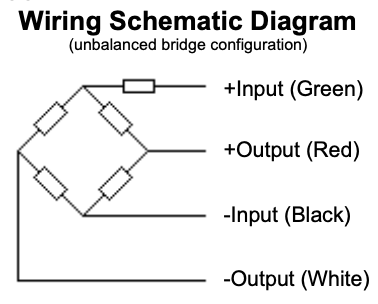
\includegraphics[width=0.3\textwidth]{load-cell-wiring.png}
	\caption{The wiring schematic for the load cell}
	\label{fig:wiring}
\end{figure}


\subsection{ADC}
To convert the millivoltage output from the load cell into a digital signal, an ADC is needed. The device used in this paper is an HX711, and apart from being a converter, it also serves as an amplifier for the load cell signal. We can see the front of the piece in figure \ref{fig:hx711}, and on the left side are the pinout where all the wires from the load cell should be connected. It's worth bearing in mind that the color coding of the wiring is not the same for all load cells, and the backside should be checked so that the connections made follow the correct wiring schematic. 

It outputs data via two of its pins, the DAT and the CLK. The CLK pin will output 0 if it's ready to send data, and 1 if it is not ready. When it is ready, the DAT pin will send  a series of 0s and 1s that can be converted from binary to a decimal value, which will then represent the output of the load scale.\cite{hx711-datasheet} Multiple code libraries have been written to handle this for the user, and the only thing left to implement is to specify which pins are being used by CLK and DAT respectively. For this paper, a library written for micropython was used.\cite{hx711-lopy}

\begin{figure}[h]
	\centering
	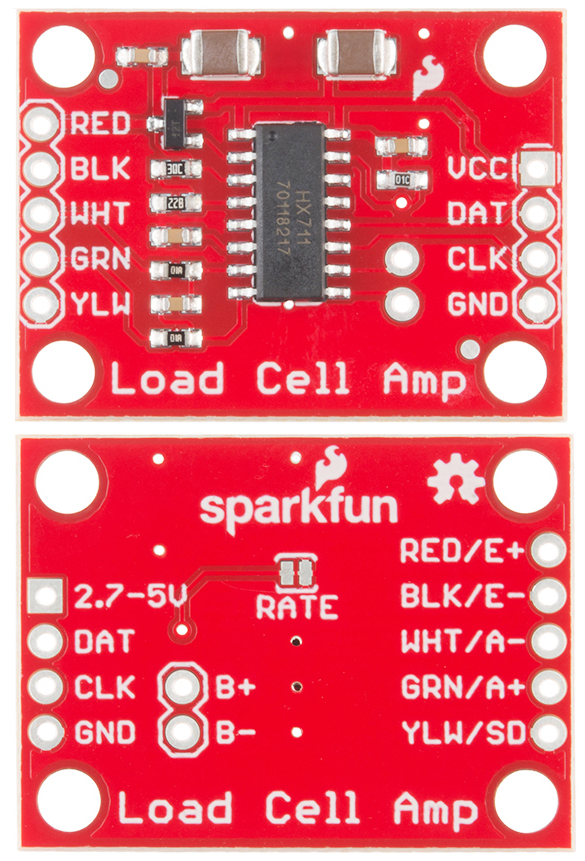
\includegraphics[width=0.3\textwidth]{hx711.png}
	\caption{The front and back of the HX711}
	\label{fig:hx711}
\end{figure}


\subsection{Microcontroller}
The microcontroller used for this paper was the FiPy development board from PyCom. It boasts a wide range of capabilities when it comes to communication protocols, NB-IoT being one of the five available.\cite{fipy-docs} With the supplied expansion board, connections via pinout is possible. It runs on micropython, which is an implementation of Python 3 optimized to run on microcontrollers.\cite{micropython}

\subsection{Power Source}
In the early stages of the project, the hardware was powered via USB cable from a computer. Since the USB was of type micro, the voltage output was at 5V. The benefit of this setup was a simple wiring schema where each component powered the next in line. The drawback was that the FiPy could only supply the ADC with 3V, which in turn affected the ADC's ability to read data from the load cell. During testing, the output rate of the raw data would be infrequent and erratic, sometimes taking several seconds to produce a single value. The values themselves did not correspond to increases and decreases in force being applied to the load cell, and would seemingly spike and crash at random. These problems were largely in part due to insufficient voltage being supplied to the ADC and load cell as later setups would reveal.

To remedy this, an approach using two different power sources was tried, where the ADC was powered by a wall outlet at a higher voltage, while the FiPy kept the USB. This resulted in electrical interference throughout the system, because of two different grounds being present in the circuit. The output rate of the data values had improved to a bit more stable rhythm than before, and the raw data values were a bit more responsive to the force applied to the load cell. 

The best setup that was tested involved an Otii battery toolbox, which is an advanced piece of hardware used to profile and emulate batteries.\cite{otii-web} With this piece of equipment, a common ground was provided to all components, as well as adequate voltage. It was capable of supplying 5V to both the FiPy and the ADC at the same time, which in turn enabled stable output of data values. When force was applied to the load cell, the data values responded accordingly with an increase or decrease in value. Due to time constraints and hardware availability, the setup could not be used for real network transmissions of the load cell data.

All data values produced by the load cell and ADC during these tests were raw values, as a calibration for kg/lb values for our intents and purposes would not bring any significant enhancements to the project.

\subsection{Wiring}
\begin{figure}[h]
	\centering
	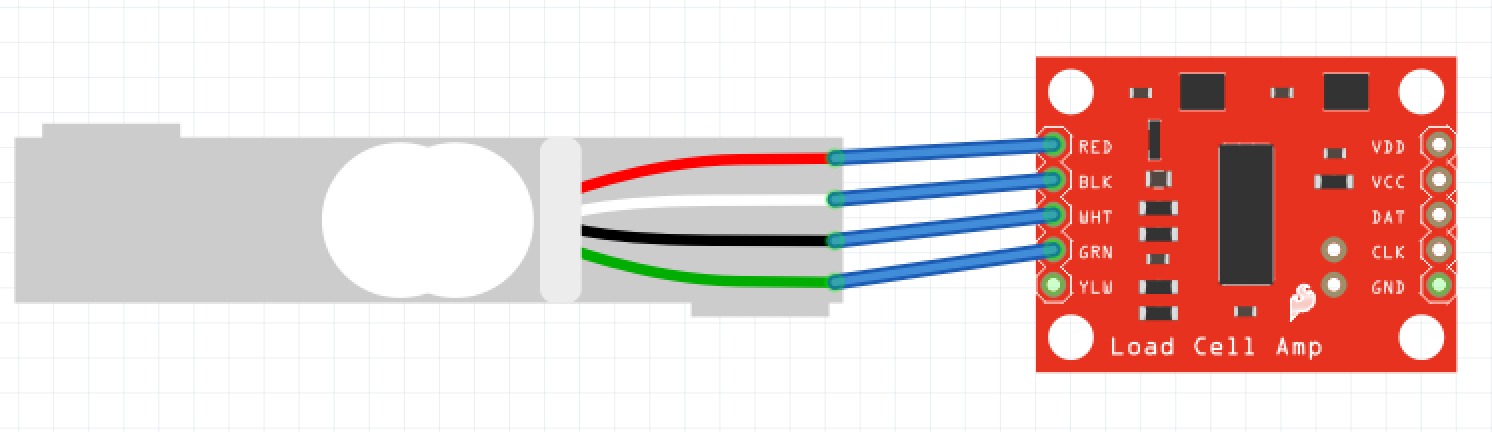
\includegraphics[width=0.6\textwidth]{load-cell_hx711.png}
	\caption{The load cell wired to the ADC}
	\label{fig:load-cell_hx711}
\end{figure}

\subsection{Failures}
During the first half of the project a faulty load cell was being used, which resulted in major delays of the hardware implementation. During the later half of the project no adequate solution to the problems with the power source could be devised in time for the practical testing of the hardware. Despite this, a short-lived setup with the Otii battery toolbox enabled a fairly functional load cell that could output tangible data values.




\section{Software Implementation}
The FiPy code runs on MicroPython, an implementation of Python 3 optimized for microcontrollers. MicroPython only executes two files on its system's root folder, the \lstinline{boot.py} and the \lstinline{main.py} files. Any remaining code must be placed in the \lstinline{lib} folder. The \lstinline{bootp.py} runs first, and is intended to contain low-level code that is meant to configure the hardware. The \lstinline{main.py} file contains the main program loop, and imports auxiliary files from the \lstinline{lib} folder.

\subsection{reader.py}
The \lstinline{reader.py} file contains the \lstinline{Reader} class, which is responsible for processing the data polled from the load cell and passing it on to being transmitted. To instantiate a functional \lstinline{reader} object, it needs to be passed a poller function as well as a transmitter function. The purpose of having these functions passed to the instance of the class instead of being hardcoded into the class is to follow the separation of concern design principle.\cite{sep-concern} The poller function should accept no argument and is expected to return the current data value produced by the load cell when called. The transmitter function in turn should accept the data value to be transmitted.

The main method of the \lstinline{reader} instance is the \lstinline{run()} method. When called, the \lstinline{run()} method performs a cycle consisting of data polling, a check for false values, adjustment of the polling rate as well as a possible transmission. 

\subsubsection{Failure Check}
The polled data value is subsequently checked for validity in the form of out-of-bounds values or extreme delta changes. A separate class called \lstinline{Fail_tracker} monitors the interval and frequency of these occurrences, and the purpose of the class is to raise an error when the error rate is deemed too high, and an administrator needs to be notified. This will result in an error message being transmitted. The internal workings of the \lstinline{Fail_tracker} will be explained in a separate section.

\subsubsection{Adjustment of polling rate}
If the value is deemed valid, it is added to a FIFO (First-in, First-out) buffer of the most recent values. The contents of the buffer are then summed into a total delta value, which is used to adjust the polling rate. If the total delta surpasses a pre-defined threshold, the polling rate is increased, whereas if it is lower it might be maintained or decreased.


\subsection{fail\_tracker.py}
The purpose of the Fail\_tracker class is to keep track of the failure occurrence and frequency. The intended usage is to instantiate an instance of the class, and call the \lstinline{strike()} method when an invalid read has occurred. This method increases an internal counter, which will then raise an exception if it passes a pre-defined threshold.

\subsubsection{GRACE\_PERIOD constant}
When invalid reads occur due to some external or internal circumstances, it might not be beneficial to count all errors within a given timeframe towards raising an exception. We are not interested in sending an alert when short periods of errors occur, instead, it is at the long-lasting periods of polling errors an exception should be raised. To account for these short bursts, we use a \lstinline{GRACE_PERIOD} constant. This constant is used for the time window after the \lstinline{strike()} method has been called, during which sequential calls  will not count towards the exception raising threshold. This time period is measured in second.

\subsubsection{COOLDOWN constant}
Since the errors 

\subsection{Data Transmissions}

\chapter{Results}
\iffalse
\begin{itemize}
	\item Don’t make the reader do all the work
	\item Have hypothesis, test them, state result clearly
	\item Two lists are not a comparison
	\item Be the first to criticize your own work
\end{itemize}
\fi


\chapter{Discussion}
\iffalse
\begin{itemize}
	\item Don't make the reader do all the work
	\item Have hypothesis, test them, state result clearly
	\item Two lists are not a comparison
	\item Be the first to criticize your own work
\end{itemize}
\fi

\chapter{Threats to Validity}
\input{chapters/7_threats}

\chapter{Conclusions \& Future Work}
\iffalse
\begin{itemize}
	\item Critique
	\item Discussion
	\item Don't make the reader do all the work
\end{itemize}
\fi


\section{Future Work}

\bibliographystyle{plainnat}
\bibliography{main}

\end{document}

%%% Local Variables: ***
%%% mode: latex ***
%%% TeX-master: "main.tex"  ***
%%% ispell-local-dictionary: "British"  ***
%%% End: ***